\chapter{Các giải pháp, đóng góp nổi bật và minh họa các
chức năng của hệ thống}
\section{Vấn đề lựa chọn công nghệ}
Có rất nhiều công nghệ bao gồm các thư viện, ngôn ngữ, frame work,
tool giúp các lập trình viên dựng lên một trang web. Mỗi một công nghệ
mới ra đời đều đáp ứng tốt nhu cầu thị trường tại thời điểm đó và
khắc phục được những nhược điểm của các công nghệ cũ. Ví dụ trước đây,
một lập trình viên front-end cơ bản chỉ cần biết về HTML, CSS sao cho
dựng lên một trang web thật đẹp, responsive đầy đủ thì nay mọi thứ đã
khác. Các website hiện nay phải động, phải linh hoạt, phải thay đổi,
phải được cập nhật để không đi lùi, vì vậy các lập trình viên front-end
hiện nay cần phải biết nhiều hơn về công nghệ, phải làm nhiều hơn.

Dựa theo xu thế công nghệ hiện nay, em chọn ReactJS – Redux để
xây dựng phần giao diện khi mà thư viện này có một cộng đồng lớn
và được Facebook phát triển. React-Router để định tuyến, xây dựng
Single Page Application, i18next để triển khai đa ngôn ngữ,
Redux-Saga để xử lý middleware, gửi request và nhận api từ back-end server. 

Về phần back-end, ban đầu em chọn Java Spring để xây dựng.
Java Spring với Maven hay Gradle hỗ trợ quản lý các gói thư viện
thêm vào (dependency), tạo sẵn dự án theo chuẩn
MVC (Model-View-Controller). Tuy nhiên trong quá trình code với
Java Spring, có nhiều vấn đề xảy ra như biên dịch Java chậm,
máy tính cá nhân chạy dự án Java Spring bị chậm, Hibernate của
Spring khó dùng các câu truy vấn SQL thông thường để giao tiếp
với cơ sở dữ liệu, … Vì vậy em chọn Go để xây dựng
lại back-end server. Về cơ bản thì Go đã khắc phục được các
nhược điểm ở trên, ngoài ra Go còn hỗ trợ tốt xử lý đa luồng với
Goroutine và Chanel đã trình bày ở phần công nghệ back-end nên
em nghĩ Go sẽ tăng hiệu năng xử lý request trong một thời
điểm (kiểm tra bằng test hiệu năng).

\section{Chức năng phân quyền động}
Phân quyền là tính năng không thể thiếu được trong các trang mang
tính chất quản trị, mỗi người cần phải được giới hạn trong truy cập.
Ví dụ không thể để một nhân viên bán hàng sử dụng được tính năng
quản lý sản phẩm hay giá sản phẩm. Do đó dựa trên các tính năng
đã phân tích như quản lý phân quyền, quản lý sản phẩm, quản lý tài khoản,
quản lý kho, quản lý tuyến bán hàng, … em phân chia người dùng
hệ thống vào các security\_group, mỗi security\_group lại có một tập
quyền (permissions). Hệ thống sẽ dựa vào các permission mà người
dùng có để xác định xem họ có thể truy
cập được vào tính năng đó hay không.

\begin{table}[H]
\centering
\begin{tabular}{| m{5cm} | m{11cm} |}
\hline
\textbf{security\_group} & \textbf{security\_permission} \\
\hline
ADMIN &
VIEW\_EDIT\_PARTY, VIEW\_EDIT\_USER\_LOGIN,
VIEW\_EDIT\_SECURITY\_GROUP,
VIEW\_EDIT\_SECURITY\_PERMISSION \\
\hline
PRODUCT\_MANAGER &
VIEW\_EDIT\_PRODUCT \\
\hline
SALES\_MANAGER & 
VIEW\_EDIT\_ORDER \\
\hline
FACILITY\_MANAGER & 
VIEW\_EDIT\_FACILITY \\
\hline
INVENTORY\_MANAGER & 
IMPORT \\
\hline
EXPORT\_MANAGER &
EXPORT \\
\hline
SALESMAN\_MANAGER &
VIEW\_EDIT\_SALESMAN \\
\hline
SALESMAN &
SALESMAN\_CHECKIN \\
\hline
\end{tabular}
\caption{Security\_group và permission tương ứng}
\end{table}

Khi một người dùng được thêm vào hệ thống, họ sẽ được cấp một
user\_login (hiểu như là username), giả sử người này là quản lý
sản phẩm thì sẽ được cấp một quyền VIEW\_EDIT\_PRODUCT, nếu người này
có khả năng quản lý rộng hơn làm được cả nhập kho thì sẽ cấp thêm
quyền IMPORT, … Đường dẫn (url) sẽ được gán theo permission để
kiểm soát truy nhập. Ví dụ PRODUCT\_MANAGER muốn xem danh sách các
sản phẩm thì phải truy cập url có dạng …/view-product,
url này chỉ được truy cập khi có quyền VIEW\_EDIT\_PRODUCT.

\section{Chức năng phân cụm cửa hàng}
Đây là một tính năng hoàn toàn mới, theo tìm hiểu và khảo sát của em
thì chưa có trên các phần mềm quản lý phân phối hiện nay. Xuất phát
từ ý tưởng các nhân viên bán hàng hằng ngày phải thăm các cửa hàng bán
lẻ. Vậy làm thế nào có thể tối ưu được quãng đường di chuyển của nhân
viên, để họ có thể di chuyển một cách dễ dàng nhất. Và em đã đưa
ra tính năng này, với mục đích là đưa ra gợi ý về các cụm
cửa hàng gần nhau, giúp người quản lý tuyến bán hàng chọn ra các
tuyến bán hàng phù hợp.

Sử dụng thuật toán phân cụm K-Means với đầu vào là N cửa
hàng bán lẻ trong hệ thống, và K cụm (do người quản lý tuyến
chỉ định). Đầu ra của thuật toán là K cụm, trong đó là vị trí
các cửa hàng gần nhau. Tuy nhiên khoảng cách sử dụng không phải là
khoảng cách Euclidean, mà là khoảng cách Haversine – công thức
tính khoảng cách giữa hai điểm trên tọa độ thực tế
(dựa trên kinh độ và vĩ độ).

Công thức Haversine tính khoảng cách giữa 2 
điểm $(x_1, y_1)$, $(x_2, y_2)$ trong không gian sử
dụng kinh độ và vĩ độ:
\begin{align*}
&\Delta x = x_1 - x_2 \\
&\Delta y = y_1 - y_2 \\
&a = \sin^2 \left( \frac{\Delta x}{2} \right)
    + \cos \left( x_1 \right) \times \cos \left( x_2 \right) 
    \times \sin^2 \left( \frac{\Delta y}{2} \right)
    \\
&c = 2 \times \arcsin \left( \sqrt{a} \right ) \\
&d = R \times c
\end{align*}
Trong đó: $x_1$, $x_2$ là kinh độ, $y_1$ $y_2$ là vĩ độ, tính bằng radian.
R là bán kính trái đất (xấp xỉ $6,371$ km). $d$ là khoảng cách cần tìm.

\section{Minh họa các chức năng của hệ thống}
\begin{figure}[H]
\centering
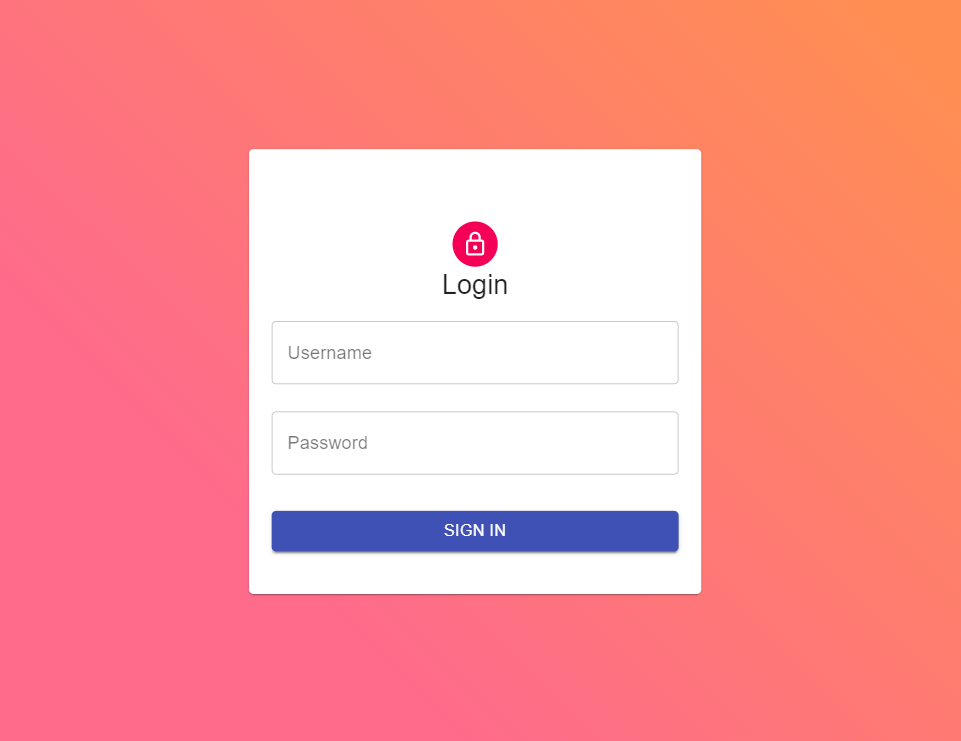
\includegraphics[width=12cm]{images/demo/login.png}
\caption{Chức năng đăng nhập}
\end{figure}

\begin{figure}[H]
\centering
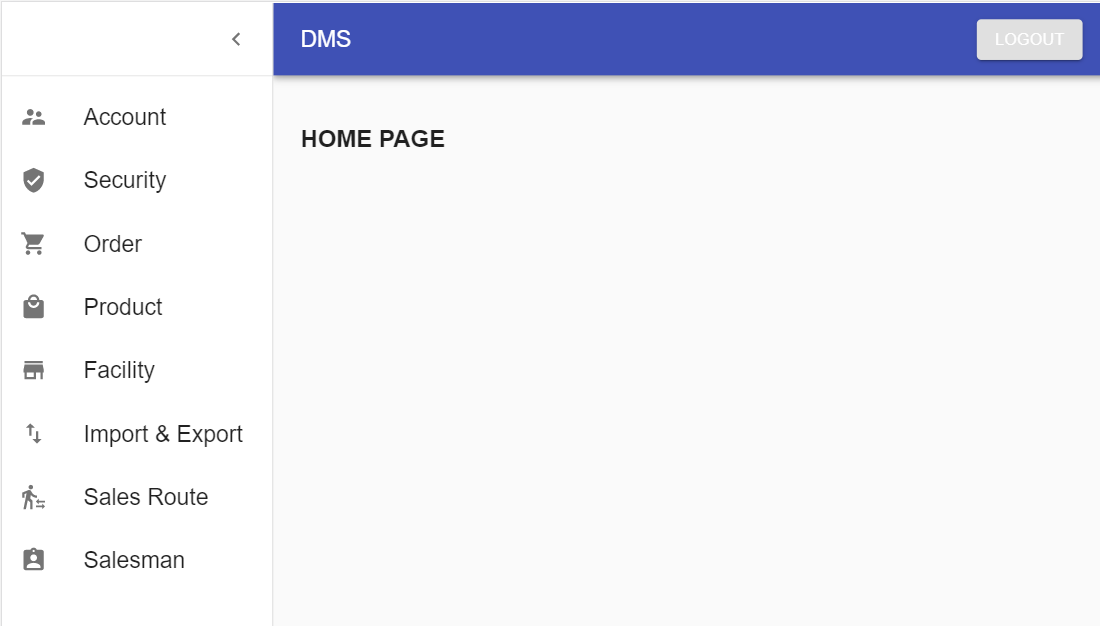
\includegraphics[width=15cm]{images/demo/home-page.png}
\caption{Giao diện trang chủ hệ thống}
\end{figure}

\begin{figure}[H]
\centering
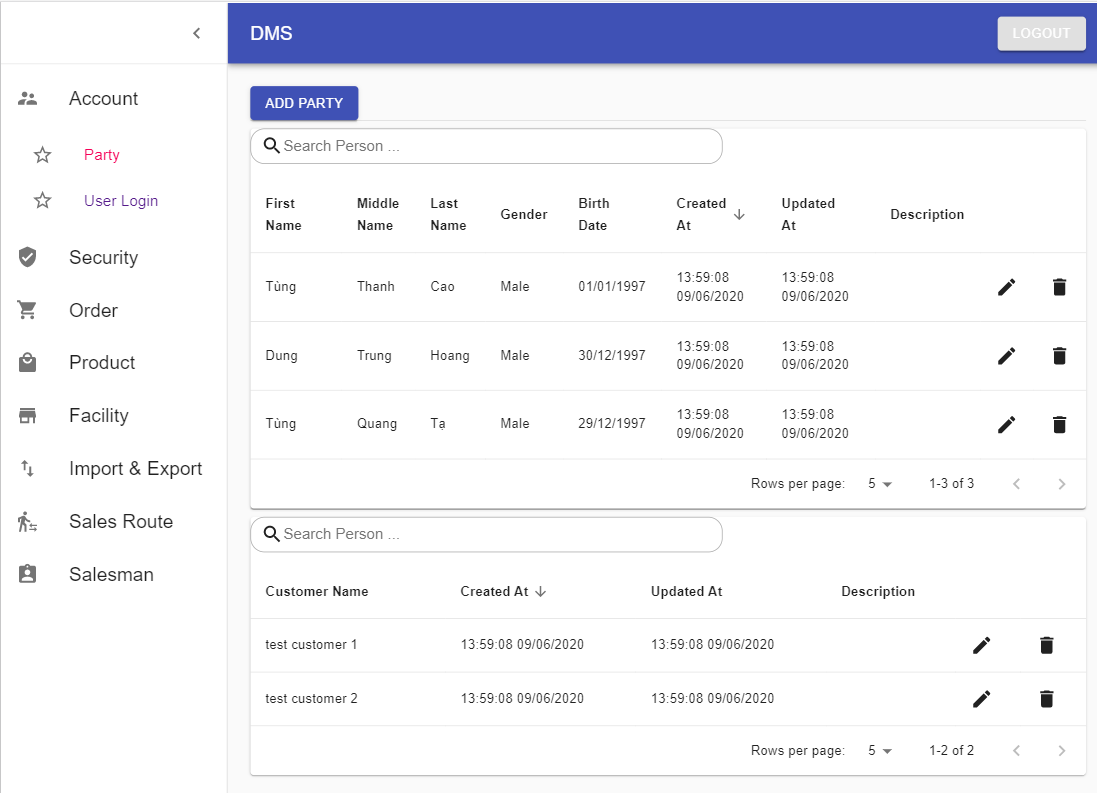
\includegraphics[width=15cm]{images/demo/party-manage.png}
\caption{Quản lý người dùng}
\end{figure}

\begin{figure}[H]
\centering
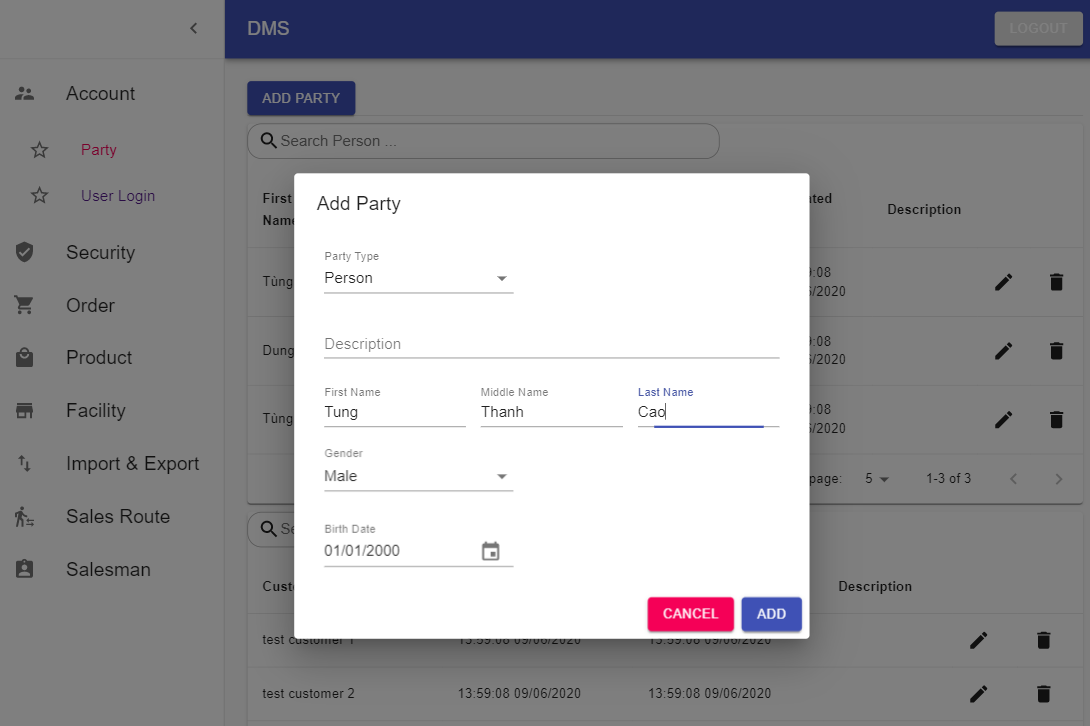
\includegraphics[width=15cm]{images/demo/add-party.png}
\caption{Thêm người dùng / khách hàng}
\end{figure}

\begin{figure}[H]
\centering
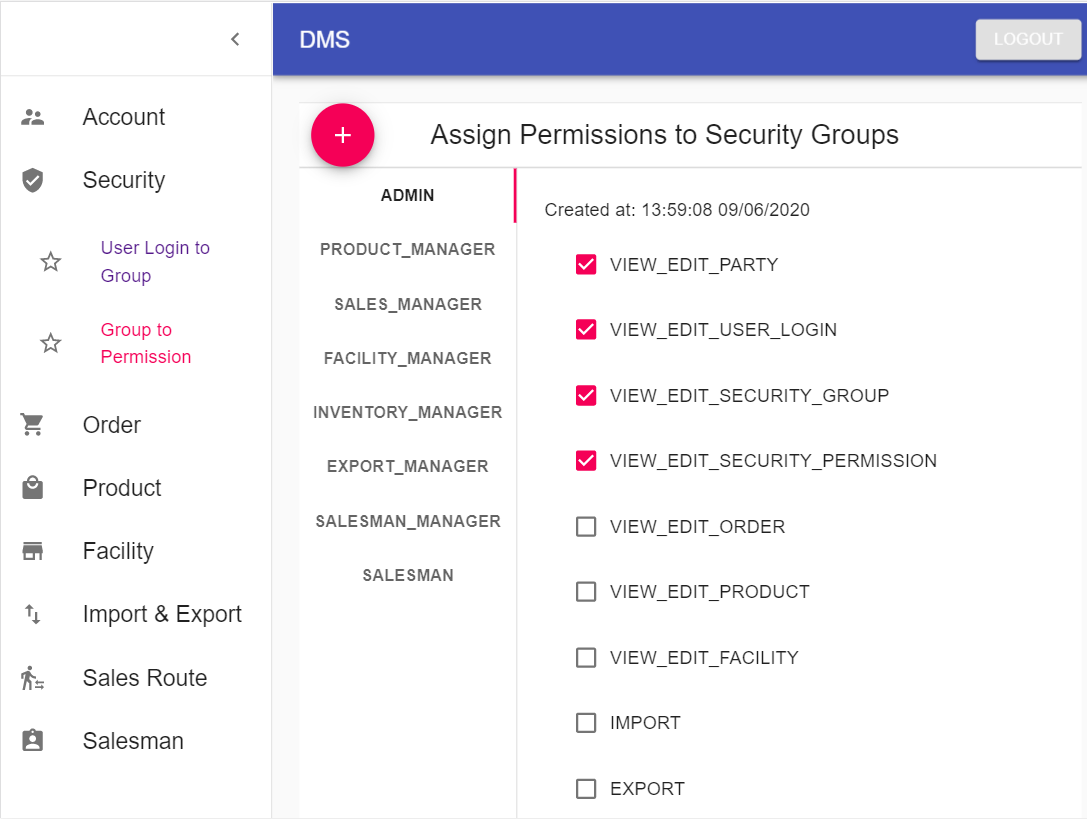
\includegraphics[width=15cm]{images/demo/group-to-permission.png}
\caption{Quản lý các nhóm quyền}
\end{figure}

\begin{figure}[H]
\centering
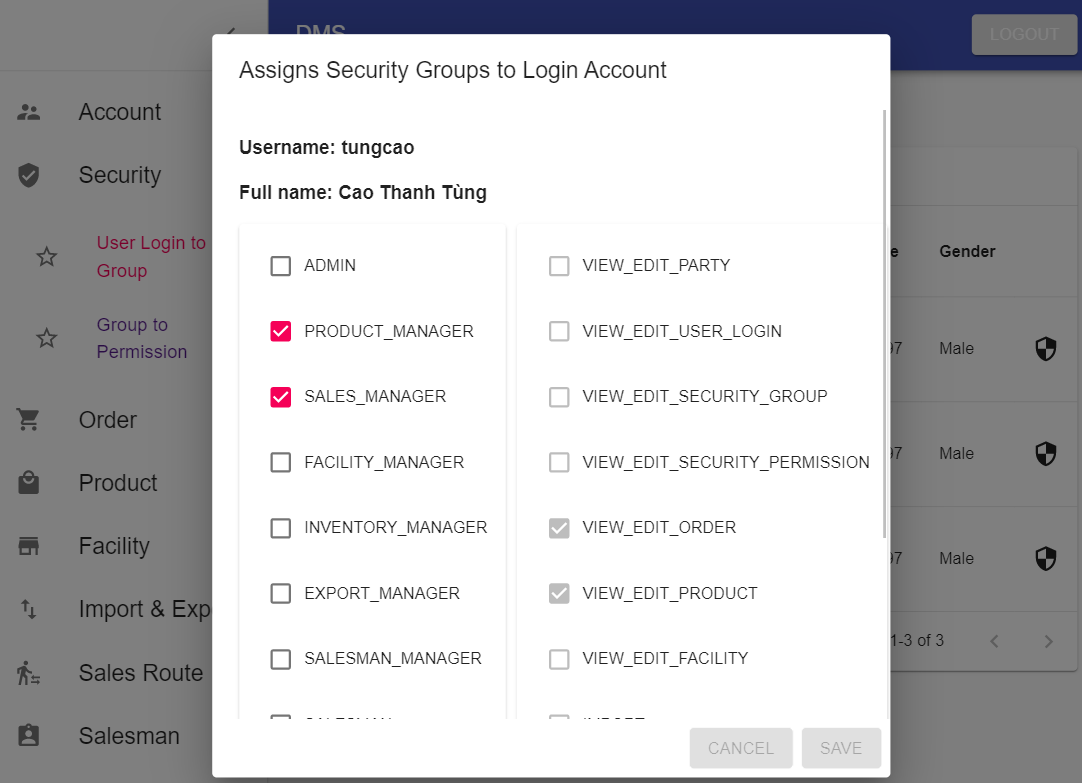
\includegraphics[width=15cm]{images/demo/user-login-to-group.png}
\caption{Gán quyền cho tài khoản người dùng}
\end{figure}

\begin{figure}[H]
\centering
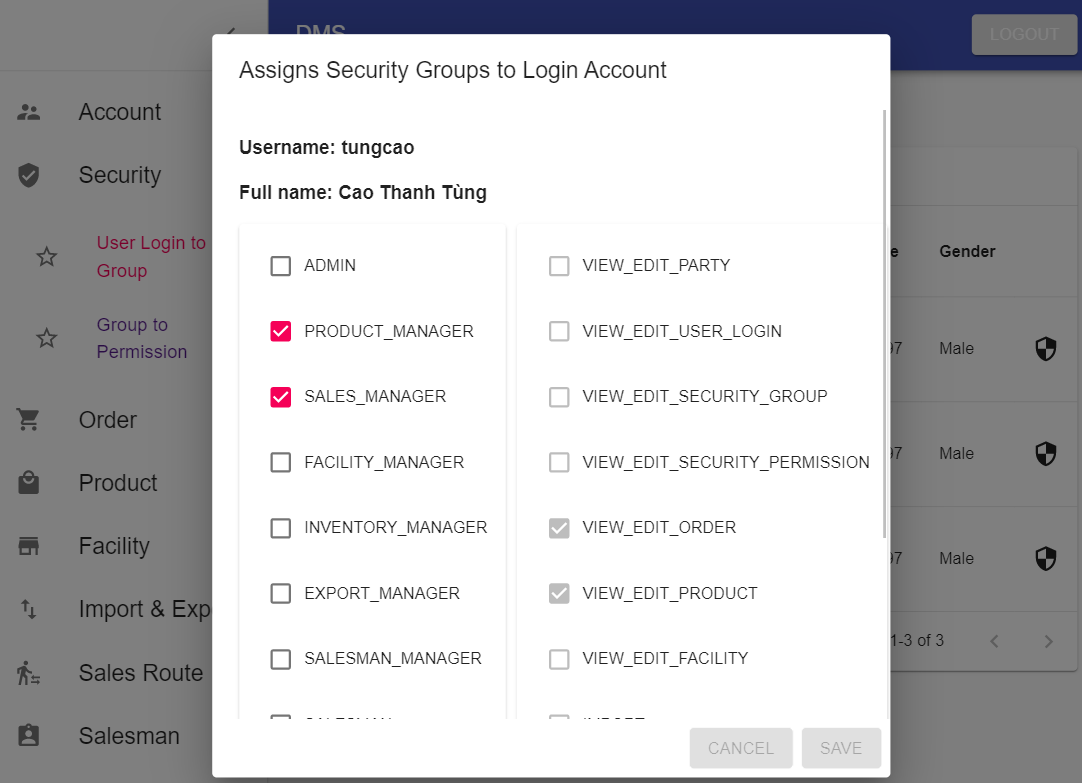
\includegraphics[width=15cm]{images/demo/user-login-to-group.png}
\caption{Gán quyền cho tài khoản người dùng}
\end{figure}

Tạo đơn hàng mới phải qua các bước như chọn khách hàng
(để giao hàng đến), chọn kho chứa hàng hóa, chọn hàng
hóa, nhập địa chỉ (nếu có hoặc chọn kho của cửa hàng).
\begin{figure}[H]
\centering
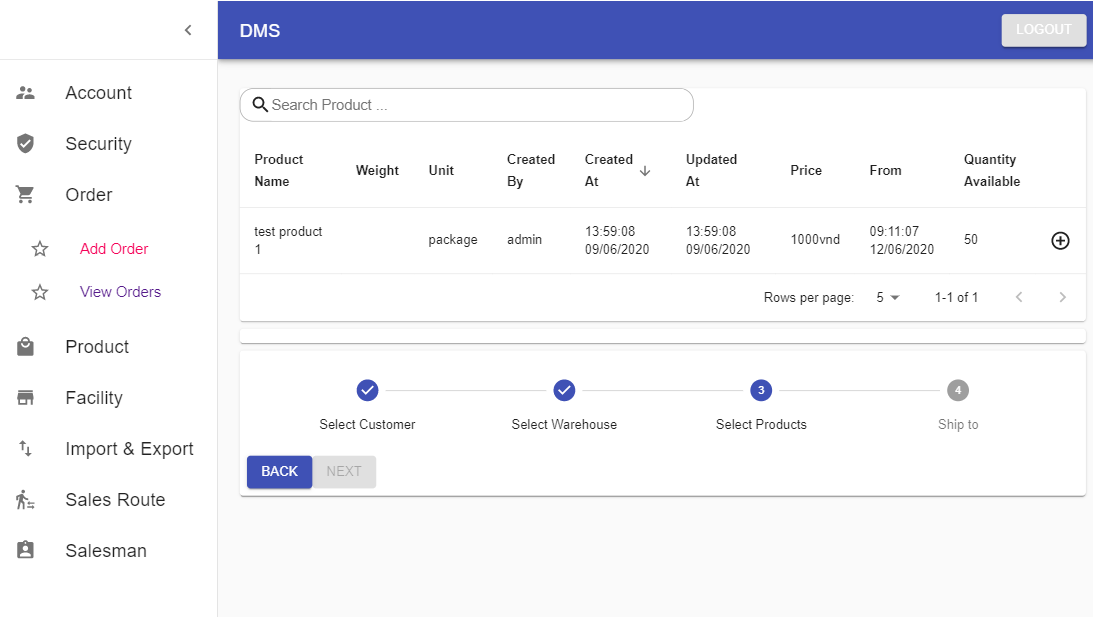
\includegraphics[width=15cm]{images/demo/add-order.png}
\caption{Tạo đơn hàng}
\end{figure}

\begin{figure}[H]
\centering
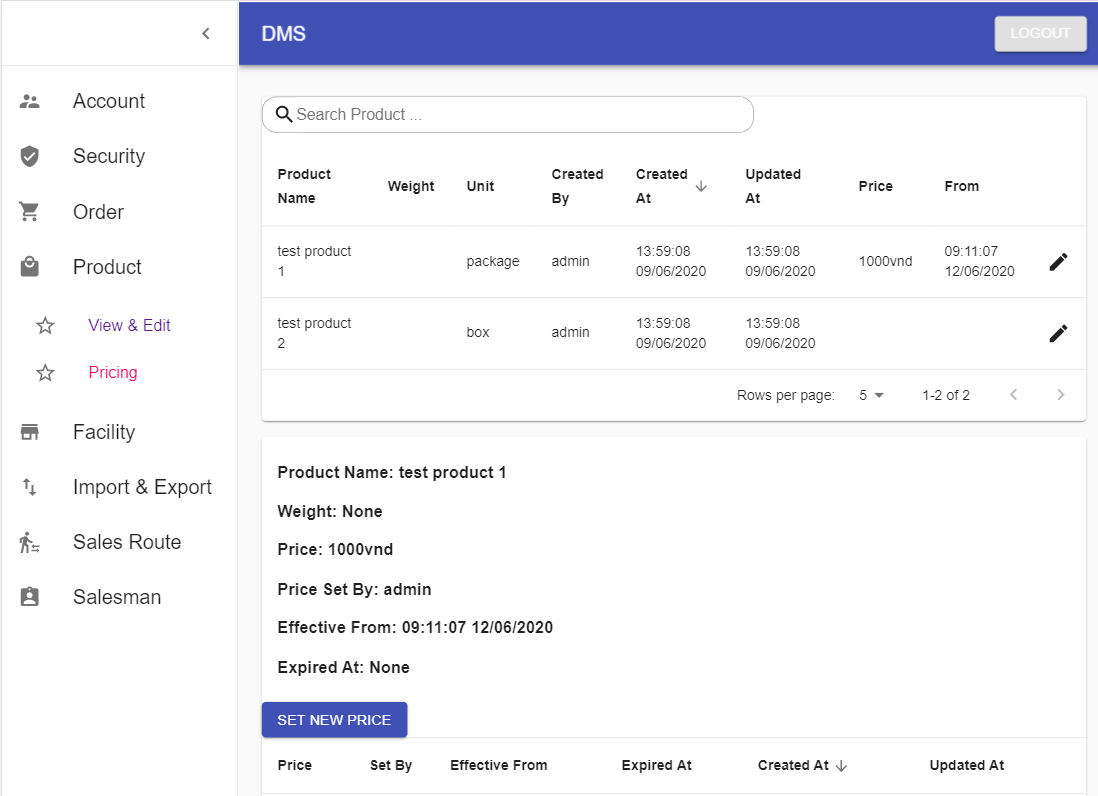
\includegraphics[width=15cm]{images/demo/product-price.png}
\caption{Quản lý sản phẩm và giá}
\end{figure}

Chức năng thêm mới cửa hàng bán lẻ, hỗ trợ bản đồ
Google Map để xác định vị trí.
\begin{figure}[H]
\centering
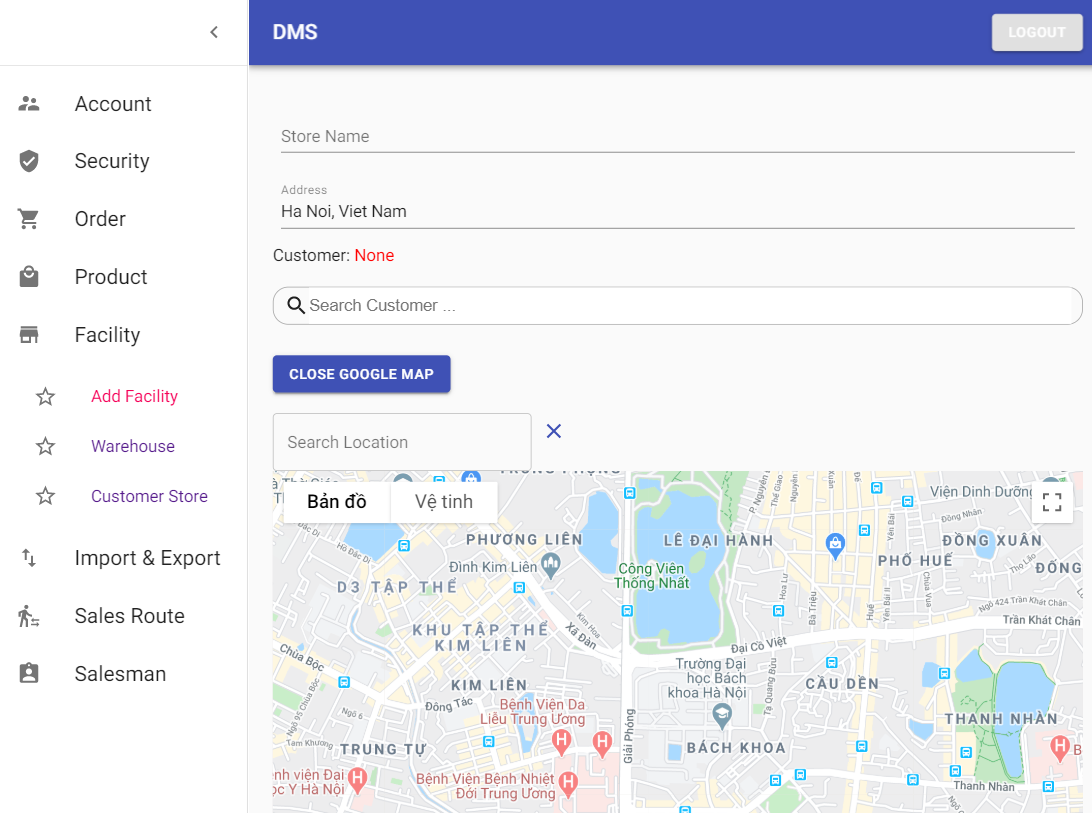
\includegraphics[width=15cm]{images/demo/add-customer-store.png}
\caption{Thêm mới một cửa hàng bán lẻ}
\end{figure}

Chức năng tạo lịch trình tuyến bán hàng, sử dụng thuật toán
K-Means phân cụm các cửa hàng bán lẻ, từ đó người quản lý
chọn ra tuyến bán hàng phù hợp nhất cho nhân viên bán hàng.
\begin{figure}[H]
\centering
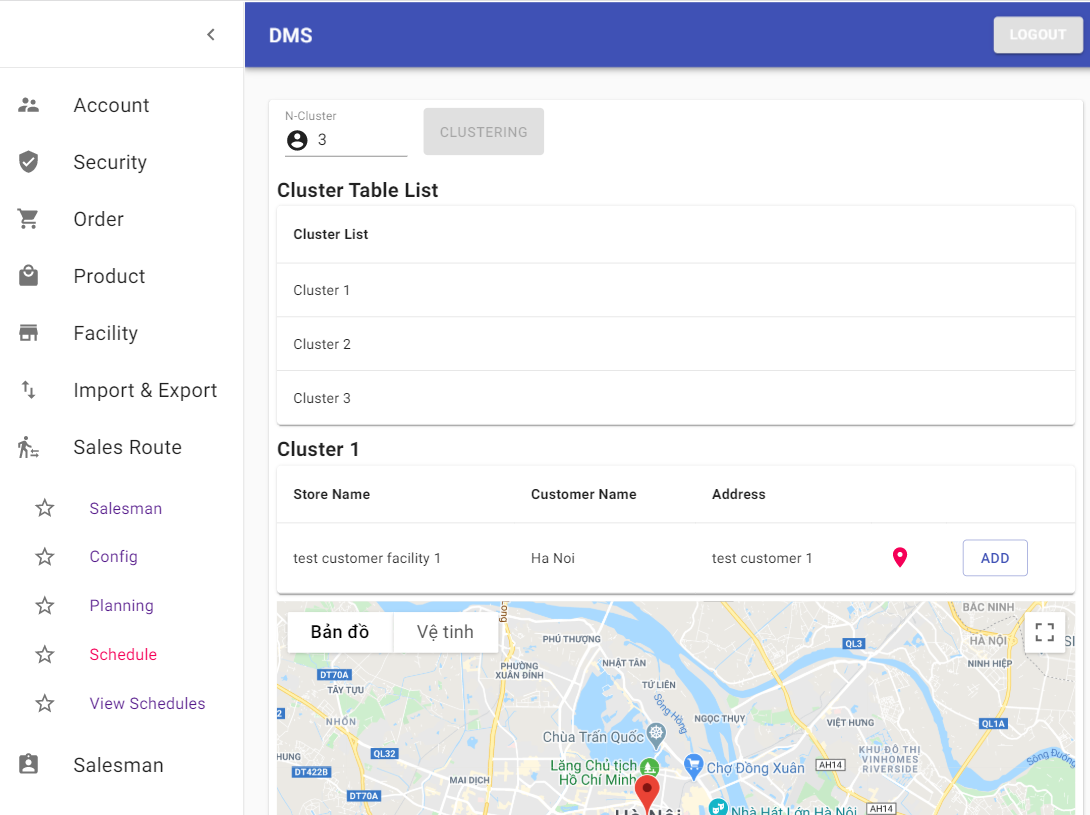
\includegraphics[width=15cm]{images/demo/add-schedule.png}
\caption{Tạo lịch trình tuyến bán hàng}
\end{figure}

\begin{figure}[H]
\centering
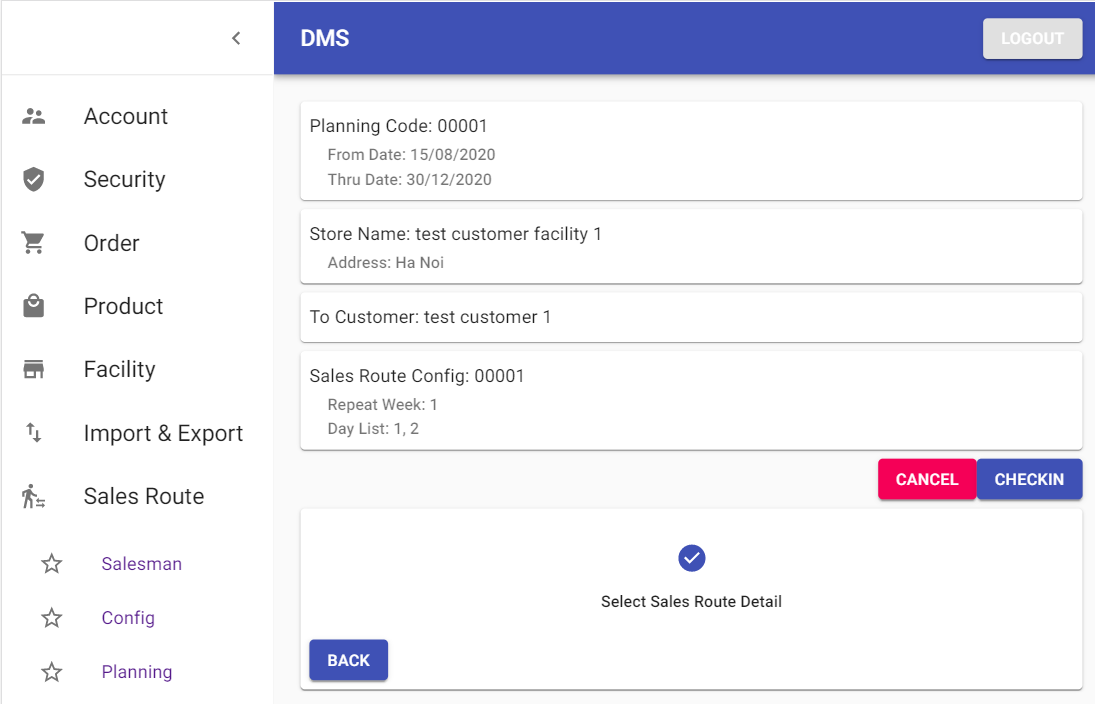
\includegraphics[width=15cm]{images/demo/salesman-checkin.png}
\caption{Salesman check-in}
\end{figure}
